% time values for run2, run4 and run5
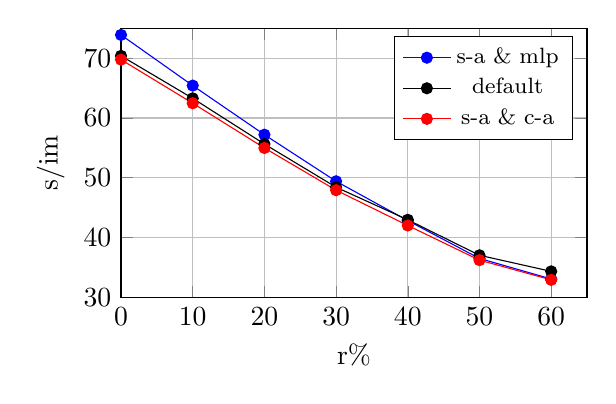
\begin{tikzpicture}
\begin{axis}[
    title={},
    height=5cm,
    width=7.5cm,
    xlabel={r\%},
    ylabel={s/im},
    xmin=0, xmax=65,
    ymin=30, ymax=75,
    xtick={0,10,20,30,40,50,60},
    ytick={30,40,50,60,70},
    legend pos=north east,
    xmajorgrids=true,
    ymajorgrids=true,
    legend style={font=\footnotesize}
]

\addplot[
    color=blue,
    mark=*
    ]
    coordinates {
    (0,73.88)(10,65.41)(20,57.20)(30,49.41)(40,42.83)(50,36.51)(60,33.08)
    };

\addplot[
    color=black,
    mark=*
    ]
    coordinates {
    (0,70.38)(10,63.28)(20,55.64)(30,48.42)(40,42.97)(50,37.04)(60,34.35)
    };
    
\addplot[
    color=red,
    mark=*
    ]
    coordinates {
    (0,69.75)(10,62.46)(20,54.98)(30,47.92)(40,42.02)(50,36.23)(60,32.93)
    };

    
\legend{s-a \& mlp, default, s-a \& c-a}
    
\end{axis}
\end{tikzpicture}